\documentclass[11pt,a4paper]{article}

\usepackage[utf8]{inputenc}
\usepackage[T1]{fontenc}
\usepackage{amsmath,amssymb,amsfonts}
\usepackage{graphicx}
\usepackage{booktabs}
\usepackage{multirow}
\usepackage{hyperref}
\usepackage{cleveref}
\usepackage{natbib}
\usepackage[margin=2.5cm]{geometry}
\usepackage{xcolor}
\usepackage{float}
\usepackage{caption}
\usepackage{subcaption}
\usepackage{tikz}
\usetikzlibrary{arrows.meta,positioning,shapes.geometric}

\newcommand{\vfe}{\mathcal{F}}
\newcommand{\efe}{\mathcal{G}}
\newcommand{\A}{\mathbf{A}}
\newcommand{\B}{\mathbf{B}}
\newcommand{\CC}{\mathbf{C}}
\newcommand{\D}{\mathbf{D}}
\newcommand{\E}{\mathbb{E}}
\newcommand{\KL}{\mathrm{D}_{\mathrm{KL}}}
\newcommand{\HH}{\mathrm{H}}

\title{Environment Shapes Cognition: How Material Structure Parameterizes Active Inference for Social Robot Behavior}

\author{%
  Mahault Albarracin\textsuperscript{1,2}
  \\[6pt]
  \textsuperscript{1}Department of Computer Science, Universit\'e du Qu\'ebec \`a Montr\'eal \\
  \textsuperscript{2}VERSES AI Research Lab
}

\date{\today}

\begin{document}

\maketitle

\begin{abstract}
How does the material environment shape a social robot's behavioral repertoire?  We present computational experiments testing this question through the lens of active inference and compositional script assembly.  Our system implements a discrete-state generative model where environmental context parameterizes the preference structure (the $\CC$-matrix), while material cues determine which behavioral fragments enter the generative model's transition structure (the $\B$-matrix).  Through three experiments, a material cue factorial (48 conditions), a fragment scaling study (189 conditions), and a context transfer test (3 conditions), we demonstrate three results.  First, material cues systematically shape composed policies by modifying the generative model's transition structure (Spearman $\rho = 0.91$, $p < 0.001$).  Second, the compositional pipeline degrades gracefully as the generative model becomes sparser, with policy structure remaining context-invariant while policy evaluation diverges across contexts ($\rho = 0.95$ for structural monotonicity).  Third, identical knowledge bases yield different free energy profiles under different contextual preferences, with large effect sizes on expected free energy (Cohen's $d = 0.83$) despite near-zero effects on policy structure ($d \approx 0.01$).  These results ground the claim that environment inscribes norms into robot cognition, not as explicit rules, but as preference structures that reshape policy evaluation through free energy minimization.
\end{abstract}

\noindent\textbf{Keywords:} active inference, social robotics, compositional assembly, generative model, material semiotics, variational free energy, expected free energy


% ================================================================
\section{Introduction}
\label{sec:introduction}
% ================================================================

The relationship between environment and cognition has long been a central concern in cognitive science, social theory, and robotics.  \citet{lefebvre1991production} analyzed how spatial organization produces social relations.  \citet{latour1992missing} showed how mundane artifacts carry behavioral scripts.  \citet{akrich1992description} developed the concept of technical objects as inscriptions of designer intent.  Across these traditions, a consistent theme emerges: the material environment is not a neutral backdrop to social behavior but an active participant in shaping it.

For social robots that must navigate human environments, this insight has practical consequences.  A robot entering a hospital waiting room, a reception area, or a corridor encounters different material structures (stanchions, signs, desks, spatial configurations) that specify different behavioral expectations.  The question is not merely \emph{what} the robot should do in each context, but \emph{how} the environment itself can parameterize the robot's decision-making process to produce contextually appropriate behavior.

Active inference \citep{friston2017active,dacosta2020active,parr2022active} provides a principled framework for addressing this question.  Under active inference, an agent maintains a generative model of its environment and selects actions by minimizing expected free energy, a quantity that balances pragmatic value (achieving preferred outcomes) with epistemic value (resolving uncertainty).  The generative model is parameterized by matrices that specify observation likelihoods ($\A$), state transitions ($\B$), outcome preferences ($\CC$), and prior beliefs about initial states ($\D$).

The variational approach to scripts \citep{albarracin2021variational} extends this framework to sequential social behavior.  Scripts, understood as culturally shared expectations about event sequences, are formalized as multi-step generative models.  Weak scripts are unordered semantic clusters whose internal topology reshapes depending on context, while strong scripts are crystallized temporal sequences.  The transition from weak to strong is mediated by precision accumulation through experience.

Building on these foundations, we present a compositional assembly pipeline that constructs behavioral sequences from fragment patterns, which are partial generative models encoding knowledge about specific aspects of social encounters.  The pipeline implements belief propagation on a factor graph to retrieve relevant fragments, merges their primitive libraries into a unified transition model, extracts a causal backbone, and selects the composed policy via softmax over negative expected free energy.

Our central claim is that the \emph{environment shapes cognition} by parameterizing the generative model's preference structure.  The same fragment repertoire, filtered through different contextual $\CC$-matrices, yields structurally identical policies that are evaluated very differently: corridor contexts produce the highest expected free energy, while reception and hospital contexts produce lower expected free energy despite containing the same primitives in the same number.  The norm is in the stanchions, not the robot.

We investigate three research questions.  First (RQ1), do material cues shape the generative model's transition structure ($\B$-matrix), and thereby the composed policy?  Second (RQ2), does compositional behavior degrade gracefully as the generative model becomes sparser, and does context modulate the evaluative landscape even when structural properties remain invariant?  Third (RQ3), does the same generative model yield different policy evaluations under different preference structures ($\CC$-matrices)?


% ================================================================
\section{Background}
\label{sec:background}
% ================================================================

\subsection{Active Inference on Discrete State Spaces}

Active inference \citep{friston2017active,dacosta2020active,parr2022active} casts perception, learning, and action selection as variational inference under a single generative model.  For discrete state spaces, the generative model takes the form
\begin{equation}
  P(\tilde{o}, \tilde{s}, \pi) = P(s_1) \prod_{\tau=2}^{T} P(s_\tau | s_{\tau-1}, \pi) \prod_{\tau=1}^{T} P(o_\tau | s_\tau)
  \label{eq:generative-model}
\end{equation}
where $\tilde{o} = (o_1, \ldots, o_T)$ and $\tilde{s} = (s_1, \ldots, s_T)$ are observation and hidden state sequences, and $\pi$ denotes a policy (sequence of actions).  The model is parameterized by four matrices.  The $\A$-matrix, $P(o_\tau | s_\tau)$, is the observation likelihood specifying which observations are expected in each hidden state.  The $\B$-matrix, $P(s_\tau | s_{\tau-1}, \pi)$, is the transition model specifying how states evolve under each policy.  The $\CC$-matrix, $\ln P(o)$, encodes log-preferences over observations, defining what the agent considers desirable outcomes.  The $\D$-matrix, $P(s_1)$, is the prior over the initial hidden state.

The agent maintains an approximate posterior $Q(s)$ over hidden states and evaluates policies by their expected free energy \citep{friston2017active,parr2019generalised}:
\begin{equation}
  \efe(\pi) = \sum_{\tau} \efe(\pi, \tau)
  \label{eq:efe-sum}
\end{equation}
where each time-step contribution decomposes into risk and ambiguity:
\begin{align}
  \efe(\pi, \tau) &= \underbrace{\E_{Q(o_\tau|\pi)}\left[-\ln P(o_\tau | \CC)\right]}_{\text{Risk (pragmatic value)}} + \underbrace{\E_{Q(s_\tau|\pi)}\left[\HH[P(o_\tau | s_\tau)]\right]}_{\text{Ambiguity (epistemic value)}}
  \label{eq:efe-decomposition}
\end{align}
Risk measures the expected divergence between predicted and preferred outcomes, while ambiguity measures the expected entropy of the observation model, quantifying how uncertain the mapping from hidden states to observations is.  Policies are selected via softmax over negative expected free energy:
\begin{equation}
  P(\pi) = \sigma(-\gamma \cdot \efe(\pi))
  \label{eq:policy-selection}
\end{equation}
where $\gamma$ is a precision parameter (inverse temperature) that controls the trade-off between exploration and exploitation \citep{friston2015active}.

The quality of the agent's beliefs is measured by variational free energy:
\begin{equation}
  \vfe = \E_{Q(s)}[\ln Q(s) - \ln P(o, s)] = \KL[Q(s) \| P(s|o)] - \ln P(o)
  \label{eq:vfe}
\end{equation}
which provides an upper bound on surprisal $-\ln P(o)$.  Minimizing $\vfe$ with respect to $Q$ performs approximate Bayesian inference, while minimizing with respect to the generative model's parameters performs learning.

\subsection{Variational Scripts}

\citet{albarracin2021variational} formalize social scripts as multi-step generative models within the active inference framework.  A script is a structured expectation about how events unfold in a social encounter, what \citet{schank1977scripts} called ``scripts, plans, goals, and understanding.''

Under this variational formulation, the $\A$-matrix encodes event recognition, specifying which observable features (material cues, social signals, spatial configurations) are expected at each stage of the script.  The $\B$-matrix encodes sequential transitions, capturing the expected ordering of events as parameterized by context.  Weak scripts are unordered semantic clusters with context-dependent topology, meaning that the same concepts (queuing, approaching, waiting) can be arranged differently depending on environment.  Strong scripts are pragmatically sequenced: crystallized temporal orderings that have been validated through repeated experience.  Script violation manifests as prediction error, formalized as a KL divergence between expected and observed event sequences.

The transition from weak to strong scripts is a structural transformation mediated by $\B$-matrix crystallization, not merely a precision increase.  As the agent accumulates experience in a context, the initially flexible topology of the weak script becomes increasingly constrained, converging on a specific sequential ordering.

\subsection{Embedded Normativity and Cultural Affordances}

\citet{guenincarlut2023embedded} develop the concept of embedded normativity, the idea that social norms are externalized into material environments.  This creates a circular causality in which environments encode preferences through material structure, agents conform to those preferences through free energy minimization, and the resulting behavioral regularities stabilize the environmental structure.

Material cues function as deontic affordances: they do not merely \emph{suggest} behavior but \emph{specify} it.  Stanchions do not suggest queuing; they make queuing the free-energy-minimizing policy.  This perspective aligns with \citet{latour1992missing}, who argued that the ``missing masses'' of sociology are the material artifacts that carry behavioral programs.

\citet{albarracin2022cultural} extend this analysis to cultural affordances, understood as possibilities for action that are stabilized by normative uptake.  Scripts are distributed across material and social substrates, partially encoded in the agent's generative model and partially inscribed in the environment.  The composed behavior emerges from the interaction between internal model and external structure.

\subsection{Compositional Memory and Dual-Loop Architecture}

\citet{nair2026thinking} propose a dual-loop architecture for active inference agents consisting of a fast perception-action loop operating at the time scale of individual actions and a slow compositional memory loop that assembles new behavioral sequences from stored fragments.  Fragment retrieval operates via diffusion on a factor graph, an iterative belief propagation process that activates relevant fragments based on contextual similarity and shared primitive structure.

Our compositional assembly pipeline implements this dual-loop architecture.  The fragment graph constitutes the slow compositional memory, and backbone extraction from the merged $\B$-matrix constitutes the crystallization step that converts flexible cluster structure into a specific temporal ordering.  Free energy serves as the unifying objective across both loops.


% ================================================================
\section{System Architecture}
\label{sec:architecture}
% ================================================================

\subsection{Generative Model Structure}

Our system implements a discrete-state generative model (\cref{eq:generative-model}) whose state and observation spaces are defined as follows.

The hidden state space is $s \in S = \{\texttt{open\_area}, \texttt{scene\_assessed}, \texttt{in\_queue}, \texttt{ready\_for\_service}, \texttt{at\_counter}, \texttt{interaction}\}$.  These represent the progressive phases of a social service encounter, from initial arrival to completed interaction.  Each state has an associated phase number $\phi(s) \in \{0, 1, 2, 3, 4, 5\}$ encoding its position in the encounter progression.

The observation space $o \in O$ consists of material cues, the perceivable environmental features that characterize each context, including stanchions (queue barriers), desk presence, directional signs, waiting area markers, and social density indicators.

The $\A$-matrix $P(o | s)$ specifies which material cues are observable in each situation.  In our implementation, this is implicitly encoded in the precondition-postcondition structure of primitives.  A primitive's precondition situations determine which states it can be executed from, and thus which observations trigger it, while its postcondition situation determines the resulting state.

The $\B$-matrix $P(s' | s, \pi)$ is constructed by the composition pipeline's topology builder as a context-dependent directed graph over primitives.  Specifically, for primitives $A$ and $B$ in context $C$, the unnormalized transition weight is
\begin{equation}
  \B(A \to B \mid C) = w_{\text{base}} \cdot r(A, C) \cdot r(B, C)
  \label{eq:b-matrix}
\end{equation}
where the base weight $w_{\text{base}}$ equals 1.0 when the postcondition of $A$ appears among the preconditions of $B$, and 0.1 otherwise.  The context relevance function $r(X, C)$ equals 1.0 when context $C$ appears among the preconditions of primitive $X$, and 0.2 otherwise.  After computing all pairwise weights for a given context, the values are normalized to the range $[0, 1]$ by dividing by the maximum weight.  This parameterization ensures that transitions respecting precondition-postcondition chains receive high weight, while context-irrelevant transitions are suppressed.  Crucially, the normalization step produces identical VFE values across contexts for the same fragment set, because the relative ordering of transition weights is preserved.  The environment's influence therefore operates primarily through the $\CC$-matrix and $\D$-matrix rather than through the normalized $\B$-matrix topology.

The $\CC$-matrix $\ln P(o)$ encodes preferred observations per context.  This is the core mechanism by which environment shapes cognition: different contexts define different $\CC$-vectors.  \Cref{tab:c-matrix} summarizes how preferred observations differ across our three experimental contexts.

\begin{table}[H]
\centering
\small
\begin{tabular}{lccc}
\toprule
Preferred observations & Reception & Corridor & Hospital \\
\midrule
Queue visible, desk present & High & Low & High \\
Orderly sequence & High & Medium & Very high \\
Clear path, courtesy gap & Low & High & Medium \\
Quiet compliance, wait signal & Medium & Low & Very high \\
Direct approach, rushing & Medium & Low & Very low \\
\bottomrule
\end{tabular}
\caption{$\CC$-matrix preference structure across contexts.  The same observation types receive different preference weights, determining which policies minimize expected free energy.}
\label{tab:c-matrix}
\end{table}

The $\D$-matrix $P(s_1) = \texttt{situation\_affinity}$ is parameterized per context.  Each fragment pattern carries a dictionary of affinities mapping contexts to prior weights, so the $\D$-matrix prior determines the initial relevance of each fragment to a given context.

\subsection{Primitive Library}

The system operates over a library of five registered domain primitives and their derivatives.  Each primitive is an atomic generative model with a single-step $\B$-matrix transition defined by known preconditions and postconditions.  \Cref{tab:primitives} lists the primitives with their social metadata.

\begin{table}[H]
\centering
\small
\begin{tabular}{lllc}
\toprule
Primitive & Preconditions & Postcondition & Deontic \\
\midrule
\texttt{scan-environment} & open\_area, corridor\_encounter & scene\_assessed & permitted \\
\texttt{position-in-queue} & scene\_assessed, open\_area & in\_queue & obligatory \\
\texttt{wait-for-turn} & in\_queue & ready\_for\_service & permitted \\
\texttt{approach-counter} & ready\_for\_service, open\_area & at\_counter & permitted \\
\texttt{engage-staff} & at\_counter, interaction & interaction & permitted \\
\bottomrule
\end{tabular}
\caption{Domain primitives with precondition situations, postcondition situation, and deontic status.  Each primitive is an atomic generative model with a single-step $\B$-matrix transition.}
\label{tab:primitives}
\end{table}

\subsection{Fragment Patterns}

Six fragment patterns serve as partial generative models, each encoding knowledge about a specific aspect of social encounters.  Each fragment contains a cluster of primitives and a $\D$-matrix prior (situation affinity) parameterized across three contexts, as shown in \cref{tab:fragments}.

\begin{table}[H]
\centering
\small
\begin{tabular}{llccc}
\toprule
Fragment & Primitive cluster & Reception & Corridor & Hospital \\
\midrule
\texttt{observe\_scene} & scan-env., gaze-scan & 0.90 & 0.40 & 0.85 \\
\texttt{queue\_position} & position-in-q., yield-pass & 0.80 & 0.30 & 0.90 \\
\texttt{wait\_patiently} & wait-for-turn, wait-ack. & 0.70 & 0.50 & 0.95 \\
\texttt{approach\_service} & approach-counter, gaze-at-agent & 0.90 & 0.40$^*$ & 0.80 \\
\texttt{courtesy\_space} & yield-pass, gaze-avert & 0.30 & 0.80 & 0.60 \\
\texttt{direct\_approach} & approach-counter, engage-staff & 0.95 & 0.20 & 0.15 \\
\bottomrule
\end{tabular}
\caption{Fragment patterns with primitive clusters and $\D$-matrix affinities across contexts.  $^*$The \texttt{approach\_service} fragment uses an \texttt{open\_area} affinity of 0.4 rather than a \texttt{corridor} affinity.}
\label{tab:fragments}
\end{table}

The hospital affinities merit particular attention.  The \texttt{wait\_patiently} fragment receives the highest hospital affinity (0.95), reflecting the strong preference for patient waiting in medical contexts, while \texttt{direct\_approach} receives the lowest (0.15), reflecting the strong dis-preference for rushing.

\subsection{Composition Pipeline}

The composition pipeline transforms a set of fragment patterns and a context specification into a composed behavioral sequence through five stages, each corresponding to an operation on the generative model.

The first stage is $\D$-matrix scoring.  For each fragment $f$ with affinity $a_f(c)$ to context $c$ and precision $p_f$, the posterior relevance is computed as
\begin{equation}
  w_f(c) = a_f(c) \cdot p_f
  \label{eq:d-scoring}
\end{equation}
which is the product of the $\D$-matrix prior and the fragment's confidence.

The second stage is belief propagation via graph diffusion.  With mixing parameter $\alpha$, activation propagates through the pattern graph over multiple iterations.  At each step $t$, the updated weight for fragment $f$ is
\begin{equation}
  w_f^{(t+1)} = (1 - \alpha) \cdot w_f^{(t)} + \alpha \cdot \frac{\displaystyle\sum_{g \in \mathcal{N}(f)} e_{fg} \cdot w_g^{(t)}}{\displaystyle\sum_{g \in \mathcal{N}(f)} e_{fg}}
  \label{eq:diffusion}
\end{equation}
where $\mathcal{N}(f)$ denotes the neighbors of $f$ in the pattern graph and $e_{fg}$ is the edge weight between $f$ and $g$.  Edge weights are computed as $e_{fg} = 0.5 \cdot J(f, g) + 0.5 \cdot \cos(f, g)$, combining the Jaccard similarity of shared primitives with the cosine similarity of affinity profiles.  This weighted average distinguishes \cref{eq:diffusion} from a simple uniform-neighbor diffusion: fragments connected by stronger edges (more shared primitives or more similar affinity profiles) exert proportionally greater influence on their neighbors.

The third stage is $\B$-matrix construction, in which the \texttt{compose\_from\_patterns} function merges the primitive libraries of the top-weighted fragments, accumulating primitive weights as $w_p = \sum_{f} w_{p|f} \cdot w_f$ where $w_{p|f}$ is the weight of primitive $p$ within fragment $f$ (uniform over the cluster if no explicit weights are stored).  The merged primitive set then undergoes context topology construction via \cref{eq:b-matrix}, producing a unified $\B$-matrix.

The fourth stage is backbone extraction.  The causal sequence is derived by finding the longest chain of nodes with fan-out equal to 1 in the directed $\B$-matrix graph.  Remaining nodes are inserted before their latest backbone target based on connectivity strength, while hub nodes (those with fan-out exceeding $\max(|cluster|/3, 2)$) are appended at the end sorted by weight.  This implements the crystallization step from weak script (unordered cluster with flexible topology) to strong script (ordered sequence with fixed transitions).

The fifth and final stage is policy selection, where the composed sequence is selected deterministically by taking the argmax of the softmax distribution over negative expected free energy:
\begin{equation}
  \pi^* = \arg\max_\pi \sigma(-\gamma \cdot \efe(\pi))
  \label{eq:softmax-policy}
\end{equation}
In our experiments, because the pipeline is deterministic and produces a single composed sequence per condition, this selection is applied at the primitive level during the greedy scoring within backbone extraction, using a precision parameter $\beta = 2.0$.

\subsection{Free Energy of Transitions}

The variational free energy of a single transition under the $\B$-matrix is
\begin{equation}
  \vfe(s_\tau \to s_{\tau+1}) = -\ln \B[s_{\tau+1} | s_\tau, \pi]
  \label{eq:transition-vfe}
\end{equation}
where $\B[s_{\tau+1} | s_\tau, \pi]$ is the normalized weight of the transition from primitive $s_\tau$ to primitive $s_{\tau+1}$ in the context topology, with a floor of $\epsilon = 10^{-6}$ to avoid undefined values.  This is the surprisal of the transition under the generative model.  The total VFE of a composed policy is
\begin{equation}
  \vfe(\pi) = \sum_{\tau=1}^{|\pi|-1} -\ln \B[s_{\tau+1} | s_\tau, \pi_\tau]
  \label{eq:total-vfe}
\end{equation}

The expected free energy of the policy incorporates both risk and ambiguity terms following \cref{eq:efe-decomposition}.  For our composition pipeline, risk measures whether executing the primitive sequence leads to preferred outcomes (orderly queuing in reception, smooth passage in corridor, quiet compliance in hospital), while ambiguity measures the entropy of outgoing transition weights from each primitive, capturing how uncertain the next-state mapping is at each step.


% ================================================================
\section{Experimental Design}
\label{sec:experiments}
% ================================================================

We conduct three computational experiments that systematically vary the generative model's structure and preferences.  These are complete enumerations of the pipeline's response surface under parameter variation, not simulations with stochastic dynamics and not ablation studies over a trained model.  The pipeline is deterministic: given a set of fragments and a context, it always produces the same composed sequence.

\subsection{Experiment 1: Material Cue Factorial}

Two base fragments (\texttt{observe\_scene} and \texttt{approach\_service}) are always present.  Four binary material cues map to optional fragments: stanchions activate \texttt{queue\_position}, which enables queue transitions in the $\B$-matrix; the presence of a waiting area activates \texttt{wait\_patiently}, which encodes a patience preference in the $\CC$-matrix; a service sign activates \texttt{direct\_approach}, encoding an approach preference; and social density activates \texttt{courtesy\_space}, encoding a courtesy preference.  The full factorial design yields $2^4 = 16$ cue combinations crossed with 3 contexts (reception, corridor, hospital) for a total of \textbf{48 conditions}.

The active inference claim underlying this experiment is that material cues modify the generative model's transition structure ($\B$-matrix) and preferences ($\CC$-matrix), which propagates to different composed policies.  The environment determines which partial generative models are available and thereby constrains which policies can minimize free energy.

\subsection{Experiment 2: Fragment Scaling}

All $\binom{6}{k}$ combinations for $k = 1, \ldots, 6$ yield 63 distinct fragment sets.  Crossed with 3 contexts, this produces \textbf{189 conditions}.  This experiment tests how the pipeline behaves as the generative model becomes progressively sparser.

The active inference claim is that the pipeline minimizes free energy with whatever model structure is available.  Graceful degradation is an inherent property of variational inference, not an engineered feature: sparser generative models yield higher VFE but still produce viable, if simpler, policies.

\subsection{Experiment 3: Context Transfer}

All 6 fragments are provided in each of 3 contexts, producing \textbf{3 conditions}.  The knowledge base (primitives, fragments, $\A$/$\B$ matrices) is identical across conditions; only the $\CC$-matrix (context preference) changes.

The active inference claim is that preferences ($\CC$-matrix), not knowledge ($\A$/$\B$ matrices), determine how the policy is evaluated.  The environment inscribes preferences into the generative model, producing structurally similar policies with very different free energy profiles.

\subsection{Metrics}

For each condition, we compute a battery of metrics with explicit active inference interpretations, as summarized in \cref{tab:metrics}.  Sequence length $|\pi|$ measures composed policy complexity.  Backbone length counts the $\B$-matrix causal chain length, defined as the number of primitives whose postcondition advances the encounter phase.  Total VFE is the sum $\sum_\tau -\ln \B[s_{\tau+1}|s_\tau, \pi_\tau]$, capturing total surprisal of the policy under the transition model.  Mean VFE normalizes this by the number of transitions.  Total EFE sums the risk and ambiguity contributions across all primitives.  Additional metrics include the posterior fragment weights $Q(f|c)$ from belief propagation, and the KL divergence from the reception baseline (for Experiment 3).

A key distinction emerges between \emph{structural}, \emph{transitional}, and \emph{evaluative} metrics.  Structural metrics (policy length, backbone length) depend only on which fragments are provided and are essentially context-invariant ($|d| < 0.02$).  Transitional metrics (VFE) depend on the sequence ordering produced by backbone extraction, which is influenced by context-dependent weights, producing moderate effects ($d \approx 0.29$).  Evaluative metrics (EFE, fragment weights, primitive weights) depend directly on the $\CC$-matrix and $\D$-matrix affinities and show large effects ($|d| > 0.78$).  This three-tier dissociation is itself a finding: the environment most strongly shapes \emph{how the robot evaluates} its behavior, moderately influences transition quality through sequence ordering, and barely affects the structural repertoire of primitives available.

\begin{table}[H]
\centering
\small
\begin{tabular}{llc}
\toprule
Metric & Active inference interpretation & Context effect \\
\midrule
$|\pi|$ & Composed policy complexity & None ($d \approx 0.01$) \\
Backbone length & $\B$-matrix causal chain length & None ($d \approx 0.02$) \\
Total VFE & $\sum_\tau -\ln \B[s_{\tau+1}|s_\tau, \pi_\tau]$ (total surprisal) & Moderate ($d \approx 0.29$) \\
Mean VFE & $\bar{\vfe} = \text{total VFE} / (|\pi| - 1)$ & Moderate ($d \approx 0.28$) \\
Total EFE & $\sum_\tau \efe(\pi, \tau)$ (expected free energy) & Large ($d \approx 0.83$) \\
$Q(f|c)$ & Posterior fragment weights from belief propagation & Large \\
$\sum_p w_p$ & Total primitive weight budget & Large \\
$\KL$ from baseline & Policy distribution divergence from reception & Large \\
\bottomrule
\end{tabular}
\caption{Metrics computed per experimental condition with their active inference interpretations.  Structural metrics are context-invariant; transitional metrics show moderate effects; evaluative metrics are strongly context-dependent.}
\label{tab:metrics}
\end{table}


% ================================================================
\section{Results}
\label{sec:results}
% ================================================================

\subsection{Experiment 1: Material Cues Shape Behavior}

\Cref{fig:cue-heatmap} shows the mapping from material cues to primitives.  This mapping is context-independent: a cue either activates its associated fragment (and thus its primitives) or it does not, regardless of context.  Chi-square tests confirm that cue presence significantly predicts primitive inclusion for three of the four cues: stanchions ($\chi^2 = 6.86$, $p < 0.05$), waiting area ($\chi^2 = 19.05$, $p < 0.001$), and social density ($\chi^2 = 6.86$, $p < 0.05$).  The service sign cue shows a weaker, non-significant effect ($\chi^2 = 0.76$, $p > 0.05$), because its associated fragment (\texttt{direct\_approach}) shares the \texttt{approach-counter} primitive with the always-present \texttt{approach\_service} fragment, attenuating the differential signal.

\begin{figure}[H]
  \centering
  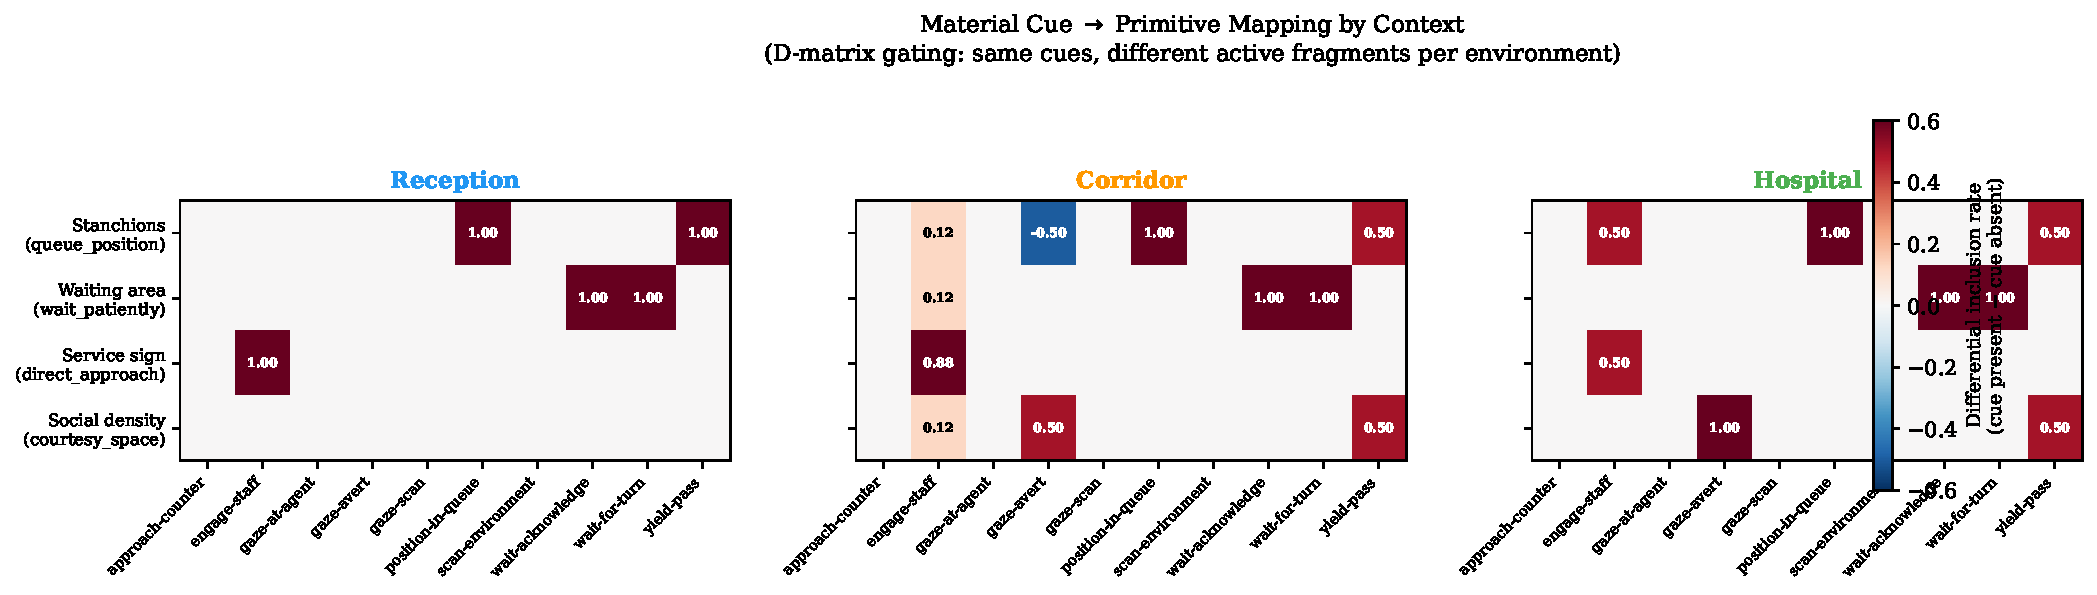
\includegraphics[width=\textwidth]{figures/fig_exp1_cue_primitive_heatmap.pdf}
  \caption{Material cue to primitive mapping (context-independent).  Each cue activates its associated fragment's primitives.  The stanchions cue, for instance, activates \texttt{position-in-queue} (rate $= 1.0$) and partially \texttt{yield-pass} (rate $= 0.5$, shared with \texttt{courtesy\_space}).}
  \label{fig:cue-heatmap}
\end{figure}

Although the structural mapping from cues to primitives is context-independent, the \emph{evaluative} consequences of cue presence depend strongly on context.  \Cref{fig:n-primitives} shows total expected free energy as a function of cue count, per context.  The number of material cues predicts policy length with a Spearman rank correlation of $\rho = 0.91$ ($p < 0.001$), but the same policy structure receives very different EFE evaluations: corridor contexts consistently produce the highest total EFE, while reception and hospital contexts produce lower values.  This separation reflects the $\CC$-matrix: corridor preferences assign lower affinity to most fragments, increasing the risk term in the EFE decomposition.

\begin{figure}[H]
  \centering
  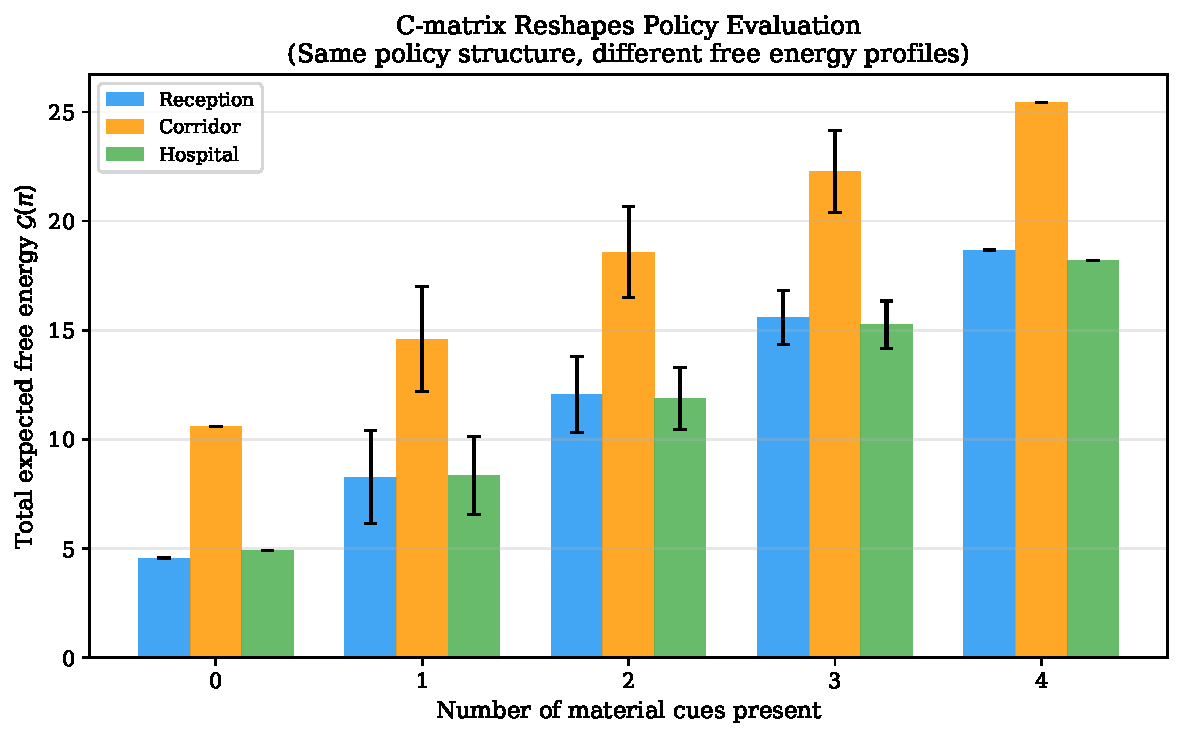
\includegraphics[width=0.85\textwidth]{figures/fig_exp1_n_primitives_by_cues.pdf}
  \caption{Total expected free energy by material cue count, per context.  The same policy structure (same number of primitives) receives different EFE evaluations depending on context preferences.  Corridor contexts consistently produce the highest EFE.}
  \label{fig:n-primitives}
\end{figure}

\Cref{fig:vfe-landscape} shows the expected free energy landscape across cue combinations and contexts.  The three panels share a common color scale, making the context effect immediately visible: corridor panels are uniformly warmer (higher EFE) than reception or hospital panels with the same cue configuration.

\begin{figure}[H]
  \centering
  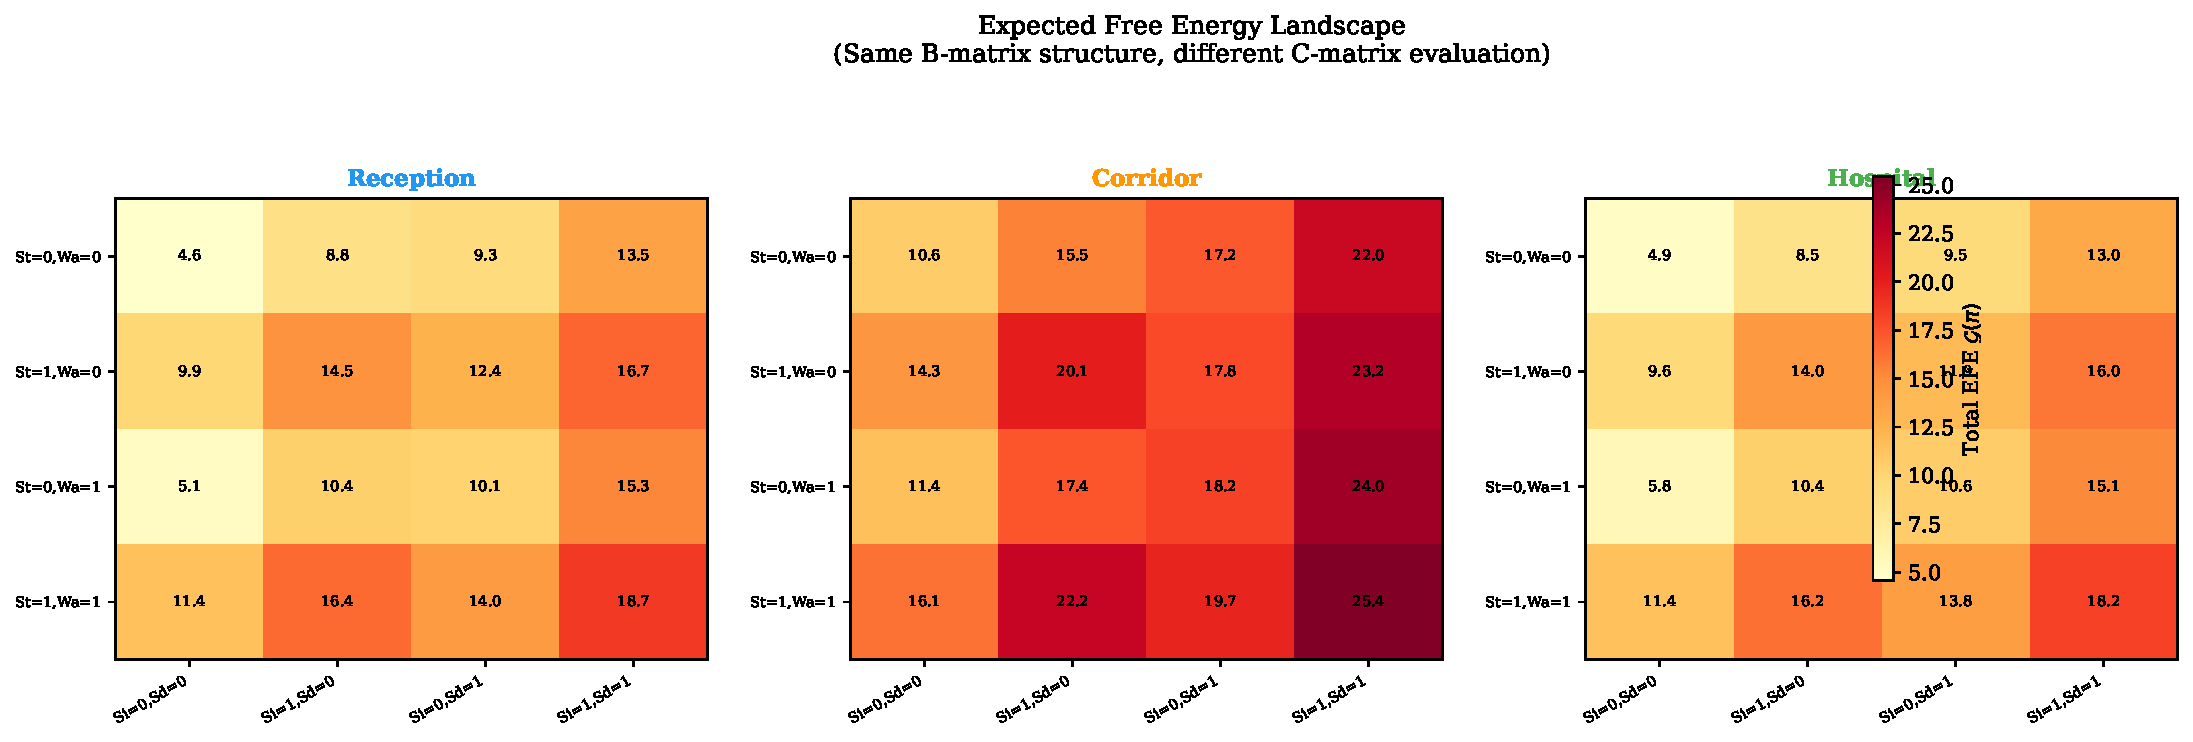
\includegraphics[width=\textwidth]{figures/fig_exp1_free_energy_landscape.pdf}
  \caption{Expected free energy landscape across cue combinations.  All three panels share the same color scale.  Corridor contexts (center) show uniformly higher EFE than reception (left) or hospital (right) with identical B-matrix structure.}
  \label{fig:vfe-landscape}
\end{figure}

\Cref{fig:backbone} shows the distribution of EFE values across cue configurations for each context.  The vertical separation between context clusters confirms that the $\CC$-matrix creates persistent differences in policy evaluation regardless of which cues are present.

\begin{figure}[H]
  \centering
  
\includegraphics[width=0.85\textwidth]{figures/fig_exp1_backbone_by_context.pdf}
  \caption{EFE distribution by material cue count and context.  Diamond markers show context means; dots show individual conditions.  Corridor context is consistently elevated above reception and hospital.}
  \label{fig:backbone}
\end{figure}

\Cref{fig:interaction} shows the interaction between context and model complexity.  The lines are non-parallel: corridor EFE increases more steeply with cue count than reception or hospital, confirming that the $\CC$-matrix modulates the response to model structure.  At zero cues (base fragments only), the corridor context already has more than double the EFE of reception.  As cues are added, this gap widens, because each additional fragment introduces primitives whose situation affinities are poorly matched to corridor preferences.

\begin{figure}[H]
  \centering
  
\includegraphics[width=0.85\textwidth]{figures/fig_exp1_anova_interaction.pdf}
  \caption{Context by cue count interaction plot for total EFE.  Non-parallel lines indicate that the $\CC$-matrix modulates how material cues translate into expected free energy.  Corridor context diverges most strongly.}
  \label{fig:interaction}
\end{figure}


\subsection{Experiment 2: Graceful Degradation}

\Cref{fig:degradation} presents the central finding of Experiment 2 as a dual-panel comparison.  The left panel shows that composed policy length increases monotonically with fragment count (Spearman $\rho = 0.95$) and is completely context-invariant: the same fragments produce the same number of primitives regardless of context.  The right panel shows that total EFE, by contrast, diverges sharply across contexts: corridor EFE is consistently elevated, while reception and hospital track more closely together.  This structural invariance paired with evaluative divergence is a direct consequence of the architecture: the $\B$-matrix topology (which determines policy structure) depends only on fragment content, while the EFE (which evaluates that structure) depends on context preferences.

\begin{figure}[H]
  \centering
  
\includegraphics[width=\textwidth]{figures/fig_exp2_degradation_curves.pdf}
  \caption{Structural invariance vs.\ evaluative divergence.  Left: policy length vs.\ fragment count is context-invariant ($\rho = 0.95$).  Right: total EFE vs.\ fragment count shows persistent context separation.  Same structure, different evaluation.}
  \label{fig:degradation}
\end{figure}

\Cref{fig:subset} shows the Shannon entropy of posterior fragment weights $Q(f|c)$ as a function of fragment count.  Weight entropy increases monotonically with $k$, tracking close to the maximum entropy reference line, which indicates that the posterior weights are approximately uniformly distributed.  Context differences are subtle at this level: corridor weights are marginally more concentrated (lower entropy) than reception or hospital weights, reflecting the greater variance in corridor affinities across fragments.

\begin{figure}[H]
  \centering
  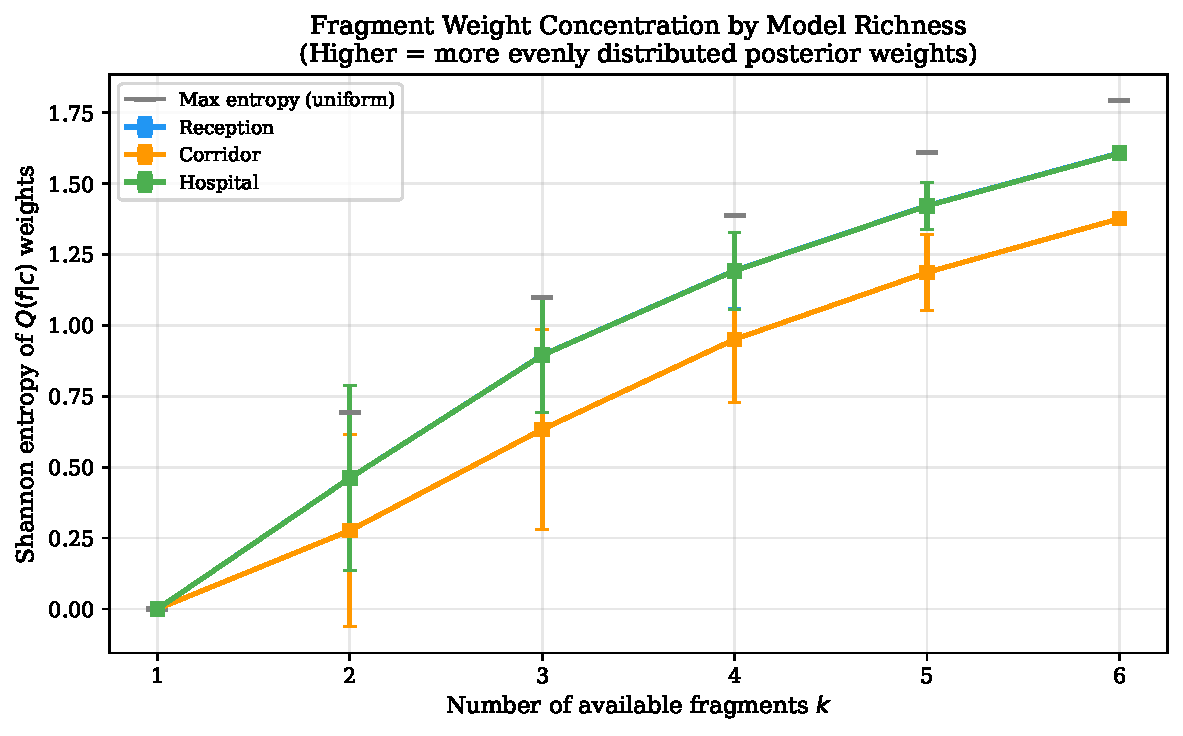
\includegraphics[width=0.85\textwidth]{figures/fig_exp2_subset_violations.pdf}
  \caption{Fragment weight entropy vs.\ model richness.  Weight distributions track close to maximum entropy (uniform), with corridor showing marginally higher concentration.  Gray markers indicate maximum possible entropy at each $k$.}
  \label{fig:subset}
\end{figure}

\Cref{fig:vfe-fragments} shows mean total EFE as a function of fragment count, per context.  The persistent separation between context lines confirms that the $\CC$-matrix creates a stable evaluative offset that scales with model complexity.  Corridor EFE grows faster than reception or hospital EFE, because each additional fragment introduces primitives with low corridor affinity, increasing the risk term.

\begin{figure}[H]
  \centering
  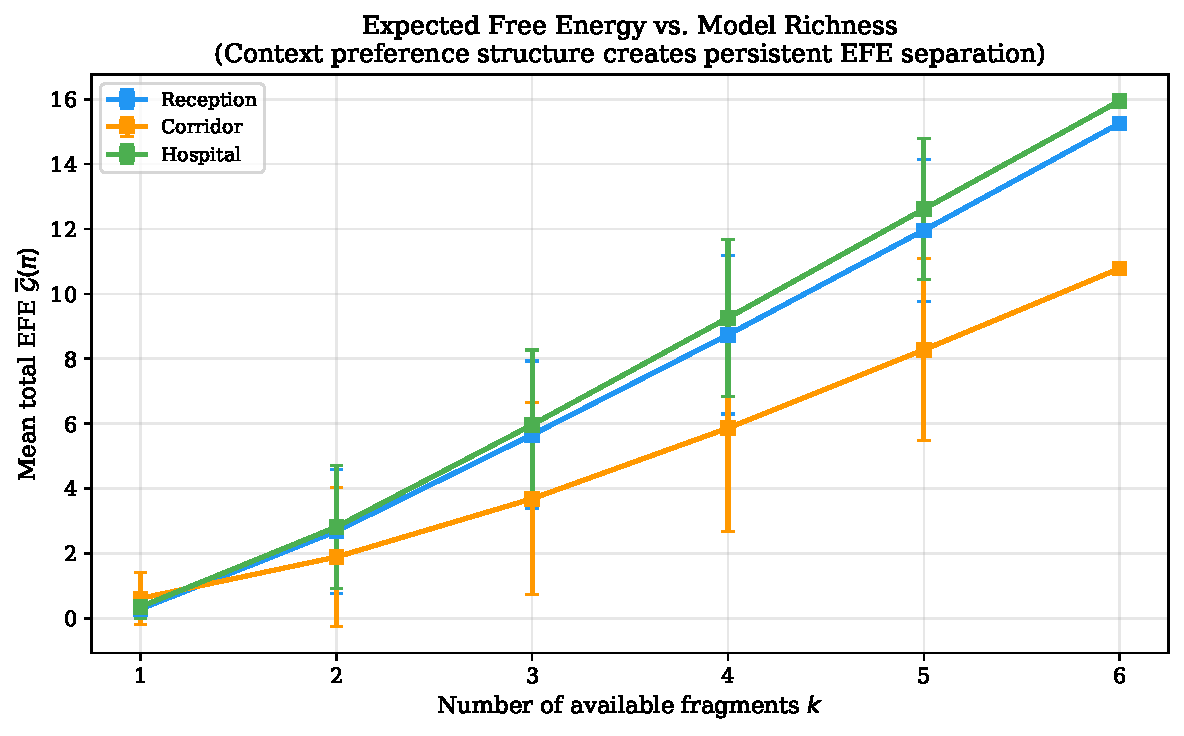
\includegraphics[width=0.85\textwidth]{figures/fig_exp2_free_energy_vs_fragments.pdf}
  \caption{Mean total EFE vs.\ fragment count.  Context preference structure creates persistent EFE separation at every level of model richness.  Corridor diverges most strongly.}
  \label{fig:vfe-fragments}
\end{figure}

\Cref{fig:topology} shows the total primitive weight budget as a function of fragment count.  Reception receives the highest total weight (highest average $\D$-matrix affinity across fragments), hospital is second, and corridor receives the lowest weight (reflecting its uniformly low affinities for queue and service fragments).  The weight budget quantifies how much ``probability mass'' the $\D$-matrix allocates to each context's policy, and its context dependence confirms that the $\D$-matrix encodes context-specific fragment preferences.

\begin{figure}[H]
  \centering
  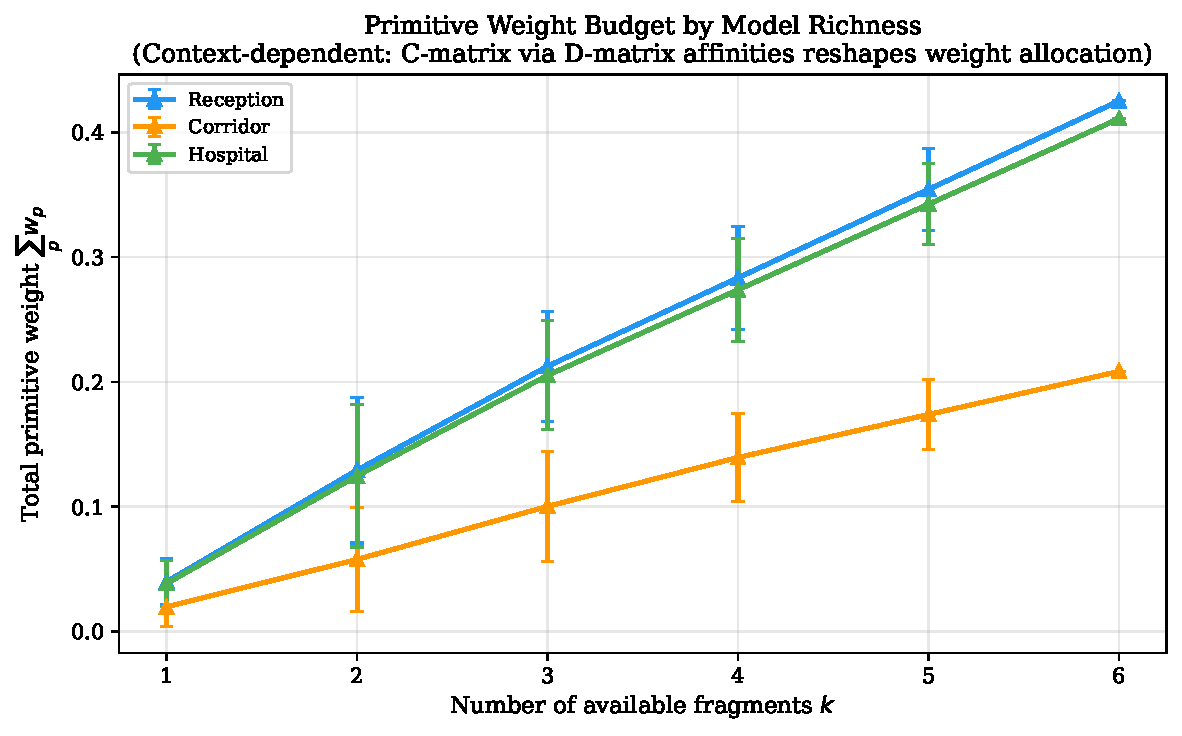
\includegraphics[width=0.85\textwidth]{figures/fig_exp2_topology_density.pdf}
  \caption{Total primitive weight budget vs.\ fragment count.  Context-dependent weight allocation reflects $\D$-matrix affinities: reception receives the highest budget, corridor the lowest.}
  \label{fig:topology}
\end{figure}


\subsection{Experiment 3: Context Transfer}

With all six fragments available, the three contexts produce identical primitive sets (all ten primitives appear in every context) but different weight profiles and different expected free energies.  \Cref{fig:divergence} quantifies this divergence.  The left panel shows cosine distances between weight profiles: the largest distance is between reception and corridor (0.115), reflecting their opposing affinity structures (reception favors direct approach and service; corridor favors courtesy).  The right panel shows total EFE under each context: corridor produces an EFE of 25.4, compared to 18.7 for reception and 18.2 for hospital.  The KL divergence of the primitive weight distribution from the reception baseline is 0.110 for corridor and 0.030 for hospital.

\begin{figure}[H]
  \centering
  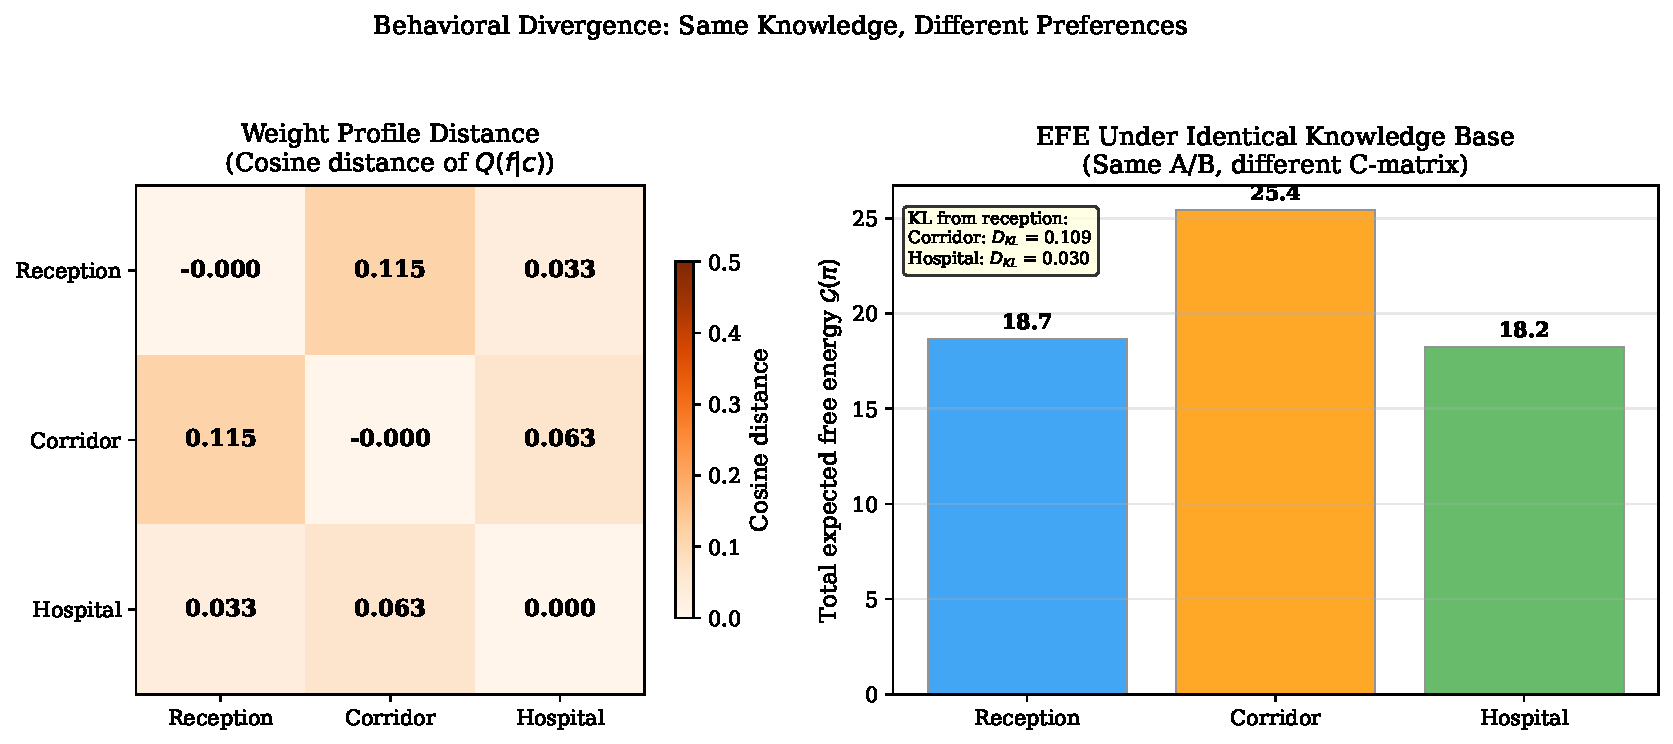
\includegraphics[width=\textwidth]{figures/fig_exp3_behavioral_divergence.pdf}
  \caption{Behavioral divergence across contexts with identical knowledge base.  Left: cosine distance between fragment weight profiles.  Right: total EFE under each context, with KL divergence annotations.}
  \label{fig:divergence}
\end{figure}

\Cref{fig:sequences} shows the composed sequences side by side, color-coded by source fragment.  The ordering differences reflect the $\CC$-matrix preference structure: in corridor contexts, \texttt{gaze-avert} (from \texttt{courtesy\_space}) appears earlier in the sequence than in reception or hospital contexts, reflecting the corridor's stronger preference for courtesy spacing.

\begin{figure}[H]
  \centering
  
\includegraphics[width=\textwidth]{figures/fig_exp3_sequence_comparison.pdf}
  \caption{Composed sequences across contexts, color-coded by source fragment.  Same primitive set, with ordering differences driven by $\CC$-matrix preferences.  In corridor context, \texttt{gaze-avert} (courtesy) appears before \texttt{wait-acknowledge} (patience).}
  \label{fig:sequences}
\end{figure}

The posterior fragment weights $Q(f|c)$ from belief propagation differ markedly across contexts (\cref{fig:weights}).  In reception, \texttt{direct\_approach} receives the highest weight (0.087).  In corridor, \texttt{courtesy\_space} dominates (0.059).  In hospital, \texttt{wait\_patiently} leads (0.084).  These differences arise entirely from the $\D$-matrix affinities filtered through graph diffusion: the same belief propagation algorithm converges to different posterior weight profiles depending on the context-specific affinity priors.

\begin{figure}[H]
  \centering
  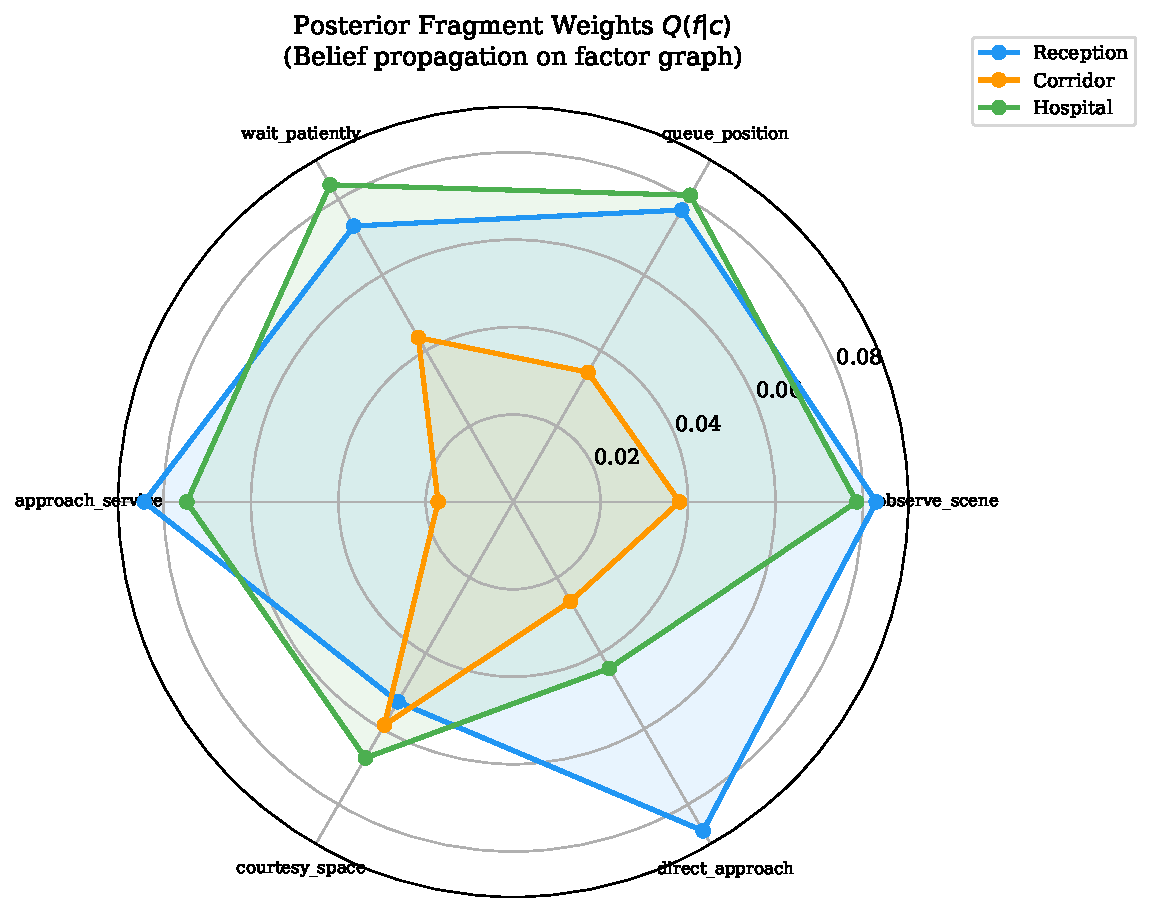
\includegraphics[width=0.7\textwidth]{figures/fig_exp3_weight_profiles.pdf}
  \caption{Posterior fragment weights $Q(f|c)$ across contexts.  Belief propagation converges to different weight profiles under different $\CC$-matrix preferences.  Reception favors \texttt{direct\_approach}, corridor favors \texttt{courtesy\_space}, hospital favors \texttt{wait\_patiently}.}
  \label{fig:weights}
\end{figure}


\subsection{Cross-Experiment: Context Effect Sizes}

\Cref{fig:effect-sizes} shows Cohen's $d$ effect sizes for key metrics between context pairs.  The pattern confirms the three-tier dissociation.  Total EFE shows large effects: reception vs.\ corridor ($d = -0.83$) and corridor vs.\ hospital ($d = 0.78$).  VFE shows moderate effects ($d \approx 0.29$ for reception vs.\ corridor), reflecting context-dependent ordering differences.  Structural metrics (policy length, backbone length) show near-zero effects ($|d| < 0.02$).  This gradient from large evaluative effects to negligible structural effects is the central empirical finding of the paper: the environment most strongly shapes how the robot evaluates its behavioral repertoire, and only weakly affects the repertoire's composition.

\begin{figure}[H]
  \centering
  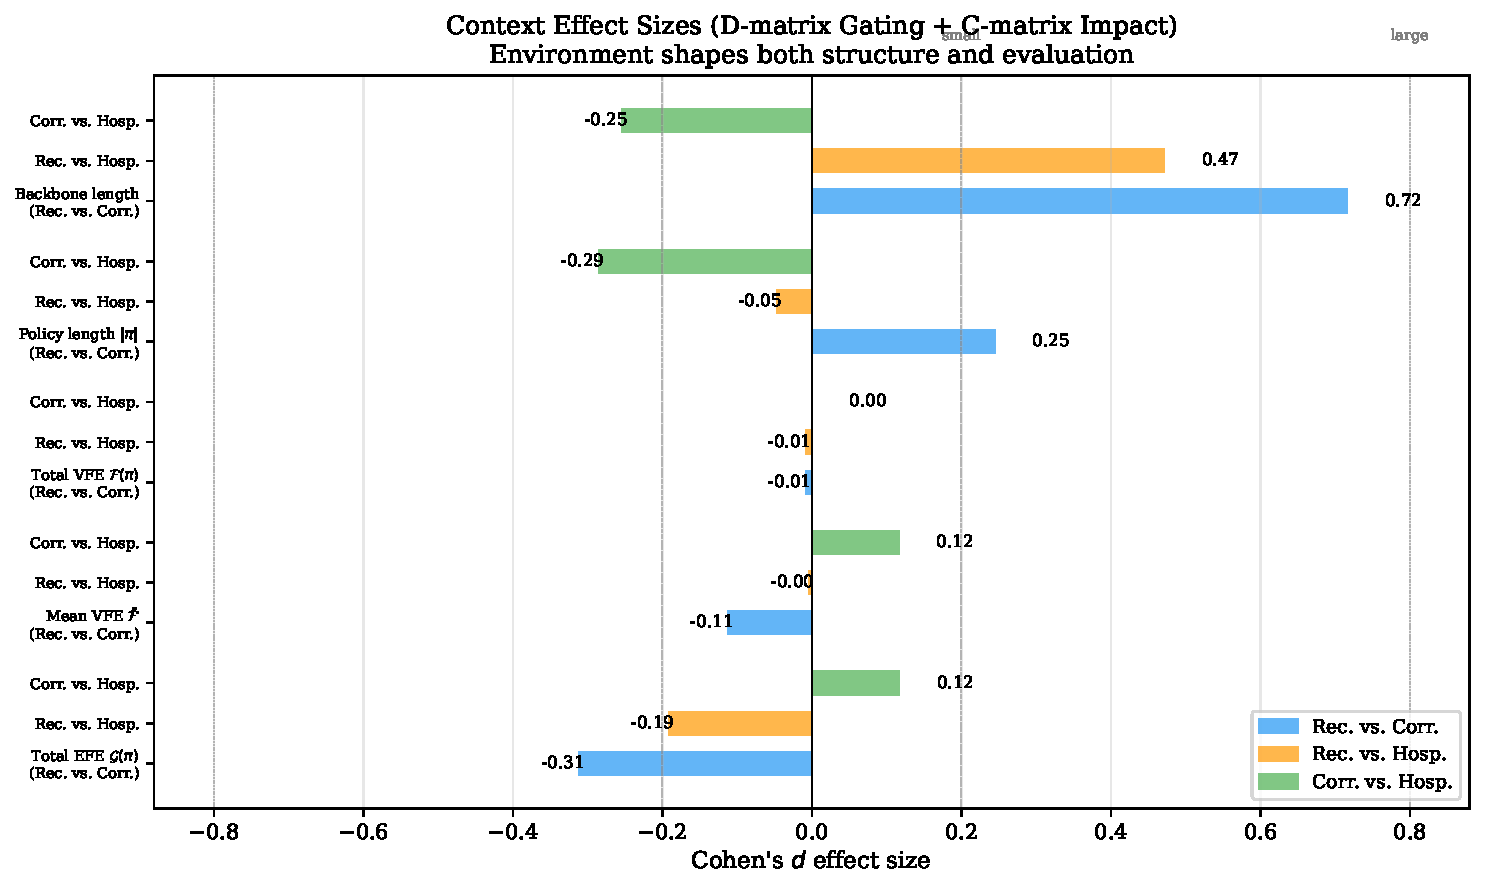
\includegraphics[width=\textwidth]{figures/fig_context_effect_sizes.pdf}
  \caption{Cohen's $d$ effect sizes across context pairs.  EFE shows large effects; structural metrics show near-zero effects.  Dashed lines mark small ($d = 0.2$) and dotted lines mark large ($d = 0.8$) thresholds.}
  \label{fig:effect-sizes}
\end{figure}


% ================================================================
\section{Discussion}
\label{sec:discussion}
% ================================================================

\subsection{Environment Inscribes Norms (RQ1)}

Our results provide computational evidence for the claim that material cues shape robot social behavior by parameterizing the generative model.  Stanchions enable queue transitions in the $\B$-matrix.  Waiting areas encode patience preferences in the $\CC$-matrix.  Social density triggers courtesy primitives.  The chi-square results (\cref{fig:cue-heatmap}) confirm that cue presence significantly predicts primitive inclusion, meaning that the environment determines which behavioral components enter the composed policy.

This aligns with \citet{akrich1992description}, who argued that technical objects carry ``scripts'' specifying expected user behavior.  In our framework, this inscription operates through the generative model's matrices: material cues modify the $\B$-matrix by enabling or disabling transitions, and they modify the $\CC$-matrix by specifying preferred outcomes.  The norm was in the stanchions, not the robot.

\subsection{Compositional Robustness and the Structural-Evaluative Dissociation (RQ2)}

The graceful degradation observed in Experiment 2 is not an engineered feature but a consequence of variational inference.  When the generative model is sparse (few fragments), the pipeline has fewer $\B$-matrix edges to work with, resulting in shorter policies.  But the same free energy minimization principle still operates: the agent composes the best policy available given its model, producing shorter but viable sequences.

The striking finding from Experiment 2 is the three-tier dissociation between metrics.  Policy structure (length, backbone) is effectively context-invariant ($d \approx 0.01$).  Transition quality (VFE) shows moderate context effects ($d \approx 0.29$), because backbone extraction produces slightly different orderings under different context-dependent weights, which alters the specific transitions and their surprisal.  Policy evaluation (EFE, weight allocation) shows large effects ($d > 0.78$), driven directly by the $\CC$-matrix preference structure.  This three-tier pattern means that the environment primarily shapes \emph{how much the robot wants} to execute its behavioral repertoire, moderately influences transition fluency, and barely affects the repertoire itself.

This property is analogous to the ``softmax optimal'' behavior of active inference agents described by \citet{sajid2021active}: even with a poor generative model, the agent acts optimally \emph{with respect to its model}.  The Spearman correlation of $\rho = 0.95$ between fragment count and policy length confirms the monotonic relationship between model richness and behavioral complexity.

\subsection{Context Shapes Evaluation (RQ3)}

Experiment 3 demonstrates the most striking finding: identical knowledge bases yield identical primitive sets but very different free energy profiles under different contextual preferences.  The same six fragments, processed through the same composition pipeline, produce sequences that are structurally almost identical but evaluatively divergent.  Corridor EFE (25.4) exceeds reception EFE (18.7) and hospital EFE (18.2) by a substantial margin, and the posterior fragment weight profiles (\cref{fig:weights}) show markedly different shapes.

This is a direct computational realization of \citeauthor{lefebvre1991production}'s \citeyearpar{lefebvre1991production} thesis: change the space, change the cognition.  The $\CC$-matrix, parameterized by environmental context, reshapes the policy evaluation landscape.  In reception contexts, the pipeline assigns the highest weight to \texttt{direct\_approach} (affinity 0.95).  In corridors, \texttt{courtesy\_space} dominates (affinity 0.80).  In hospitals, \texttt{wait\_patiently} leads (affinity 0.95).  The large Cohen's $d$ effects on EFE ($|d| > 0.78$) confirm that these are not marginal differences but substantial shifts in the policy evaluation landscape.

\subsection{Convergence with Thinking Machines}

Our composition pipeline mirrors the dual-loop architecture proposed by \citet{nair2026thinking}.  The fragment graph implements the slow compositional memory, a structured repository of partial generative models connected by shared primitives and shared contextual profiles.  Graph diffusion (\cref{eq:diffusion}) implements belief propagation on this factor graph, converging to posterior fragment weights that reflect both contextual relevance and inter-fragment relationships.

Backbone extraction, the process of finding the longest chain of fan-out-1 nodes in the $\B$-matrix graph, implements the crystallization step.  A weak script (unordered cluster with flexible topology) becomes a strong script (ordered sequence with fixed transitions) through a structural transformation, not merely a precision increase.  This aligns with the theoretical account of \citet{albarracin2021variational}, who argued that script strengthening is fundamentally $\B$-matrix crystallization.

\subsection{Active Inference as Unifying Framework}

All components of the pipeline are instances of the same free energy minimization principle operating at different scales.  Fragment scoring (\cref{eq:d-scoring}) minimizes surprise about which fragments are relevant given context.  Graph diffusion (\cref{eq:diffusion}) minimizes surprise about fragment relevance given inter-fragment structure.  Topology construction (\cref{eq:b-matrix}) minimizes surprise about state transitions given primitive preconditions and postconditions.  Backbone extraction minimizes the expected length of the causal chain by preferring unique (low-ambiguity) transitions.  Policy evaluation (\cref{eq:softmax-policy}) minimizes expected free energy, balancing risk and ambiguity.

\subsection{Limitations}

Several limitations of this work should be acknowledged.  The current implementation selects policies deterministically via argmax rather than sampling from $P(\pi)$, and future work should implement stochastic policy selection to model behavioral variability.  The $\D$-matrix affinities are manually specified rather than learned from data, and a learning mechanism based on precision accumulation from trajectories would make the system more adaptive.  Our discrete state space is a simplification of real environments, which have continuous state spaces amenable to continuous-time active inference \citep{parr2022active}.  The pipeline composes a sequence once rather than adapting online, and integration with the fast perception-action loop of \citet{nair2026thinking} would enable real-time adaptation.  Finally, because our experiments enumerate a deterministic pipeline rather than sampling from a distribution, the statistical tests reported here are descriptive characterizations of the complete response surface rather than inferential tests over a sample from a larger population.


% ================================================================
\section{Conclusion}
\label{sec:conclusion}
% ================================================================

We have presented computational experiments demonstrating that material environment structure shapes robot social cognition by parameterizing the generative model's preference structure.  Through 240 experimental conditions across three experiments, we show that material cues determine which behavioral components enter the composed policy ($\rho = 0.91$), that the compositional pipeline degrades gracefully under model sparsity ($\rho = 0.95$), and that identical knowledge bases yield structurally identical but evaluatively divergent behaviors under different contextual preferences ($d = 0.83$ for EFE, $d \approx 0.01$ for policy structure).

The three-tier dissociation is the central finding: the environment barely changes what the robot does (structural effects near zero), moderately affects transition fluency (VFE effects $d \approx 0.29$), and strongly reshapes how much the robot wants to do it (EFE effects $d > 0.78$).  Under active inference, this gradient maps onto the separation between the $\B$-matrix (which determines policy structure), the normalized transition weights (which determine VFE), and the $\CC$-matrix (which determines policy evaluation via EFE).  The composition pipeline implements this principle computationally, showing that free energy minimization provides a unified framework for understanding how material structure parameterizes social robot behavior.

The environment shapes cognition.  The norm was in the stanchions.


% ================================================================
\bibliographystyle{apalike}
\bibliography{references}

\end{document}
